%Inicio de Preámbulo

\documentclass[letterpaper,12pt]{extarticle}
\usepackage[utf8]{inputenc}
\usepackage[spanish,mexico]{babel}
\usepackage{amsmath,amssymb,amsfonts,latexsym,cancel}
\usepackage{hyperref}
\usepackage[pdftex]{graphicx}
\usepackage{wrapfig}
\DeclareGraphicsExtensions{.pdf, .png, .jpg, .PNG, .JPG, .eps, .gif}
\usepackage[rflt]{floatflt}
\usepackage{fancyhdr}
\usepackage{mathptmx}
\usepackage{float}
\usepackage{longtable,multirow,booktabs}
\usepackage{cite}
\usepackage{wrapfig}
\usepackage[square,numbers]{natbib}
\usepackage{multicol}
\usepackage{caption}
\usepackage[]{sidecap}
\usepackage{adjustbox}
\usepackage{parskip}
\usepackage{tikz}
\usepackage{lipsum}
\usepackage[table,xcdraw]{xcolor}
\setlength{\parindent}{12pt}
\u
%Fin de Préambulo

%Inicio formato de Página

\textheight = 21cm %Medidas de la  página
\textwidth = 18cm  %Medidas de la página
\topmargin = -2cm  %Medidas de la página    
\oddsidemargin = -0.8cm %Medidas de la página
\pagestyle{fancy} %Diseño de la página
\lhead{Facultad de Ingeniería}%%LeftHead
\chead{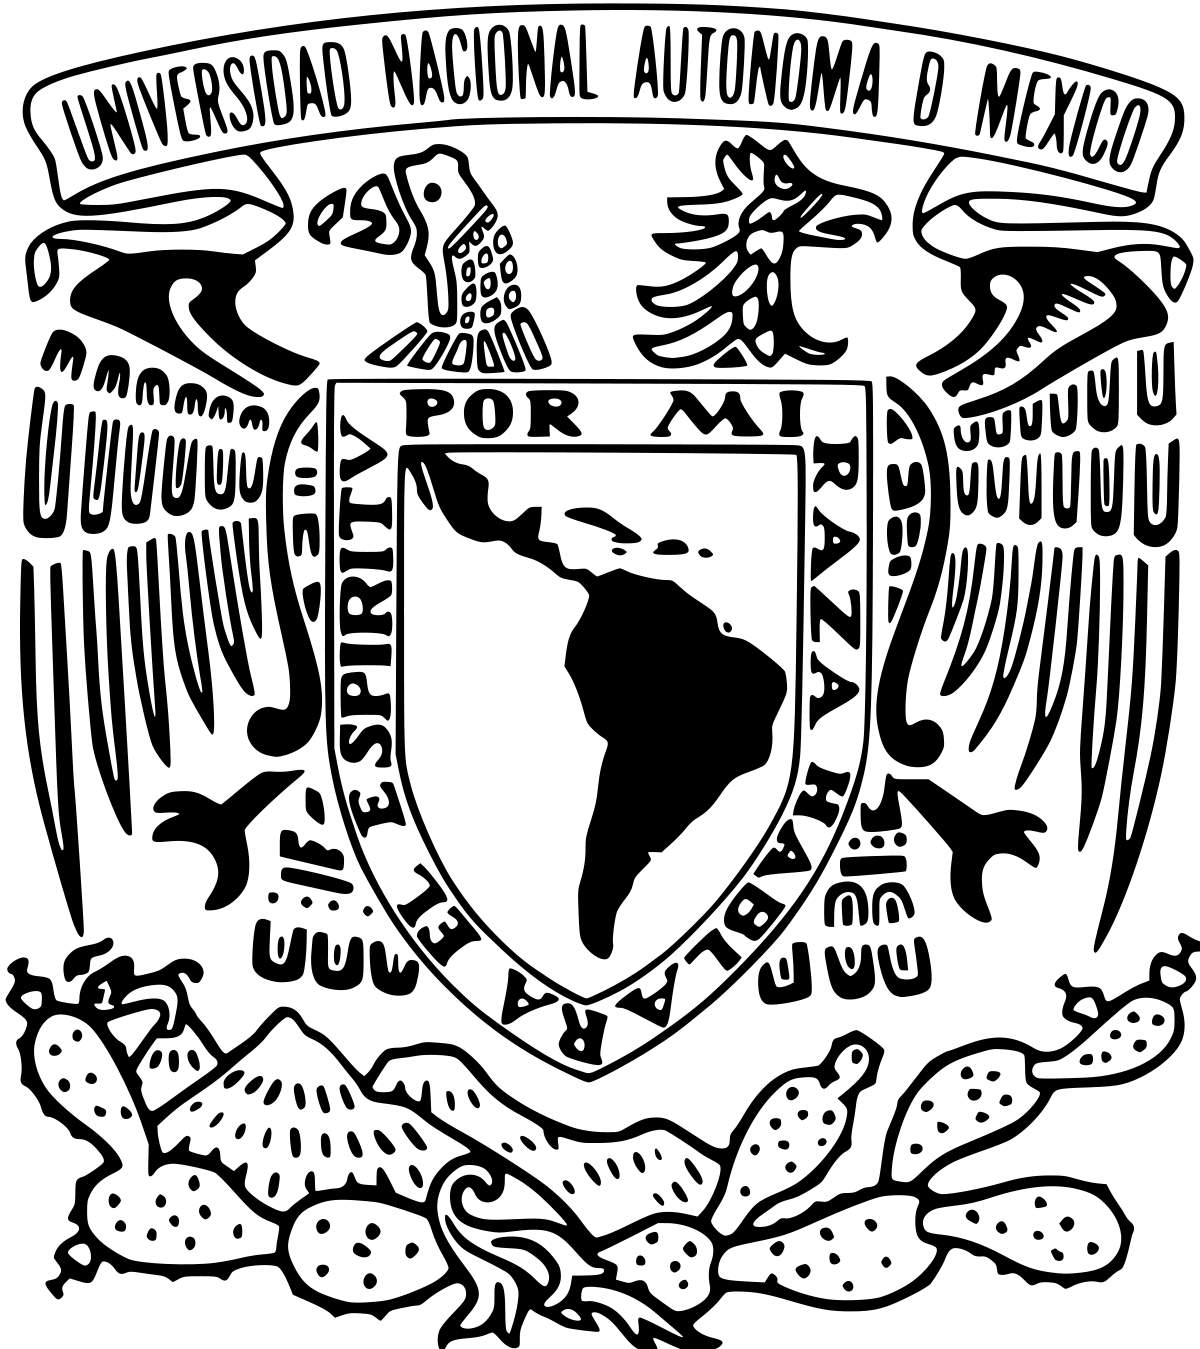
\includegraphics[width=1cm, height=1cm]{Imágenes/UNAM.png}}%%CenterHead
%\lfoot{USM}
\rhead{Estructura de Datos y Algoritmos II}%%RightHead

\setlength{\columnsep}{4mm}%Comandos para el formato de la página.
%\setlength{\parindent}{4em}%Sangría al comenzar un nuevo párrafo.
\setlength{\parindent}{0.5in}
%\setlength{\parindent}{4em}%Sangría al comenzar un nuevo párrafo.
\setlength{\parskip}{1em}%Distancia entre párrafos.
\renewcommand{\baselinestretch}{1.0}% Espacio entre línea y línea.
\setlength{\headheight}{33pt}

%Fin formato de Página

\begin{document}

\centering\Large\textbf{Manual de usuario: Ordenamiento Externo.}

\justifying\normalsize	
\section{Menú inicial}

 \noindent El menú inicial del programa permite seleccionar entre 3 opciones diferentes de ordenamiento: Polifase, Mezcla Natural y Radix. Así mismo, permite terminar la ejecución del programa seleccionando la opción (4).

\begin{figure}[h!]
\centering
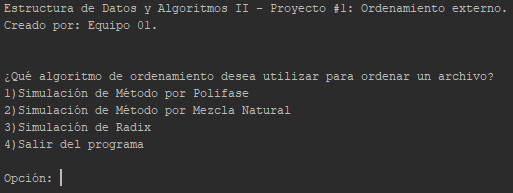
\includegraphics[height=5cm]{Imágenes/Menu1.png}
\caption{\textit{Menú inicial de selección.}}
\label{fig:Menu1}
\end{figure}

En caso de que se introduzca un número entero que no represente ninguna de las opciones presentes, el menú imprimirá un error en pantalla. Así mismo, si se introduce una entrada no númerica o un número no entero, el programa arrojará una excepción y terminará su ejecución. Evite tal situación con el fin de obtener resultados correctos.

\begin{figure}[h!]
\centering
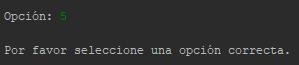
\includegraphics[height=2cm]{Imágenes/Menu2.png}
\caption{\textit{Mensaje de error recibido por una selección incorrecta.}}
\label{fig:Menu2}
\end{figure}

\section{Polifase}

\subsection{Procedimiento previo a la ejecución}
\label{section:2.1}

\noindent Al introducir esta opción en el menú inicial, se deberá de ingresar el nombre del archivo que contiene las claves \textbf{sin la extensión .txt}. Si existe un archivo con el nombre introducido en la carpeta \textit{Archivos} del programa, el procedimiento previo a la ejecución continuará. En caso contrario, recibirá un mensaje de error.


\begin{figure}[h!]
\centering
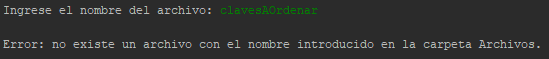
\includegraphics[height=1.5cm]{Imágenes/Poli1.png}
\caption{\textit{Mensaje de error recibido al introducir un archivo inexistente en la carpeta Archivos.}}
\label{fig:Poli1}
\end{figure}

Posteriormente, se deberá de introducir el criterio de ordenamiento deseado para las claves que serán ordenadas con los números enteros indicados como opciones de selección.

\begin{figure}[h!]
\centering
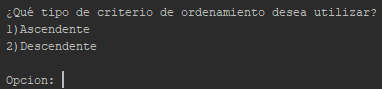
\includegraphics[height=2cm]{Imágenes/Poli2.png}
\caption{\textit{Submenú de selección para el criterio de ordenamiento.}}
\label{fig:Poli2}
\end{figure}

En caso de que se introduzca una opción entera no presente en el submenú, el programá imprimirá un error en pantalla y regresará al menú inicial.

\begin{figure}[h!]
\centering
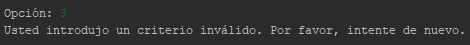
\includegraphics[height=1.25cm]{Imágenes/Poli3.png}
\caption{\textit{Submenú de selección para el criterio de ordenamiento.}}
\label{fig:Poli3}
\end{figure}

A continuación, se deberá de especificar el campo que se desea ordenar de cada una de las claves (Nombre, Apellido y Número de Cuenta) con las opciones numéricas en pantalla.

\begin{figure}[h!]
\centering
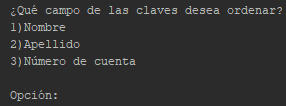
\includegraphics[height=2.5cm]{Imágenes/Poli4.png}
\caption{\textit{Submenú de selección para el campo a ordenar de las claves.}}
\label{fig:Poli4}
\end{figure}

\begin{figure}[h!]
\centering
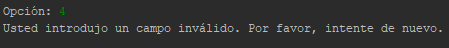
\includegraphics[height=1.25cm]{Imágenes/Poli5.png}
\caption{\textit{Mensaje de error obtenido al ingresar una opción no presente en el submenú.}}
\label{fig:Poli5}
\end{figure}

\pagebreak

\subsection{Ejecución}

\noindent Una vez que se haya realizado lo anterior, el programa comenzará a realizar el proceso inicial de lectura, generación de bloques y escritura para, finalmente, imprimir las claves ordenadas en pantalla.

\begin{figure}[h!]
\centering
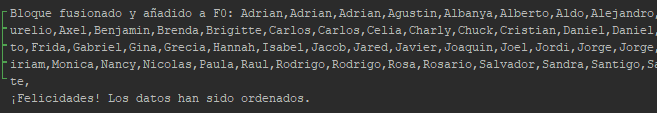
\includegraphics[height=2.5cm]{Imágenes/Poli6.png}
\caption{\textit{Salida obtenida con un archivo de 100 claves ordenadas de forma ascendente por Nombre.}}
\label{fig:Poli56}
\end{figure}

Puede verificarse el resultado en el contenido del archivo \textit{F0} generado en la carpeta \textit{Archivos $->$ Polifase}; el cuál contiene las claves ordenadas en el último bloque del mismo.

\begin{figure}[h!]
\centering
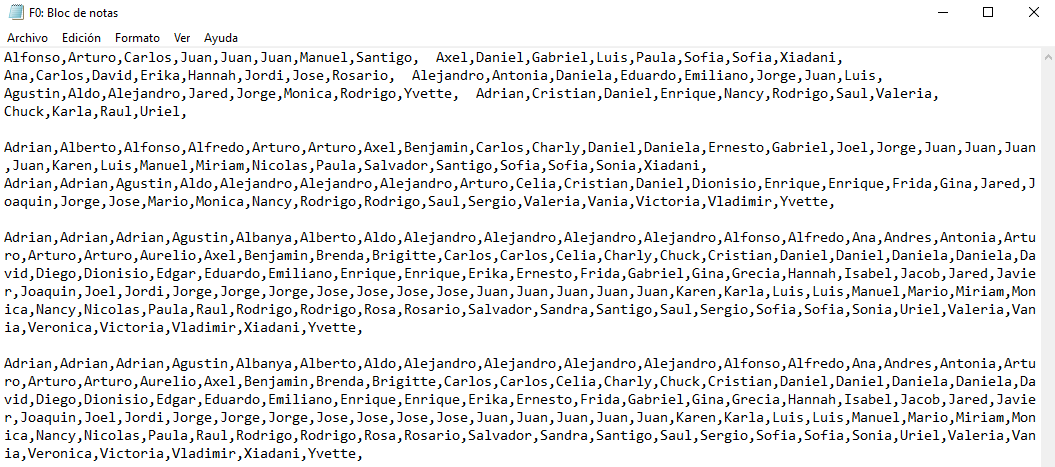
\includegraphics[height=7.8cm]{Imágenes/Poli7 .png}
\caption{\textit{Contenido del archivo F0 tras ejecutar el programa.}}
\label{fig:Poli56}
\end{figure}

Si se desea ordenar otro archivo con el formato correcto, únicamente deben de seguirse los pasos anteriores. Es importante señalar que, en caso de que el ordenamiento por Polifase se inicie de nuevo, el programa ejecutará un recolector de basura interno que reinicializará los archivos \textit{F0, F1, F2 y F3} de la subcarpeta \textit{Polifase} provenientes de ejecuciones anteriores.

\section{Radix Externo}

\subsection{Procedimiento previo a la ejecución}

\noindent Al introducir esta opción en el menú inicial, se deberá de ingresar el nombre del archivo que contiene las claves \textbf{sin la extensión .txt}. Si existe un archivo con el nombre introducido en la carpeta \textit{Archivos} del programa, el procedimiento previo a la ejecución continuará. En caso contrario, recibirá un mensaje de error.


\begin{figure}[h!]
\centering
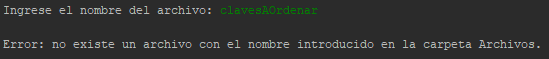
\includegraphics[height=1.5cm]{Imágenes/Poli1.png}
\caption{\textit{Mensaje de error recibido al introducir un archivo inexistente en la carpeta Archivos.}}
\label{fig:Poli1}
\end{figure}

Posteriormente, se deberá de introducir el criterio de ordenamiento deseado para las claves que serán ordenadas con los números enteros indicados como opciones de selección.

\begin{figure}[h!]
\centering
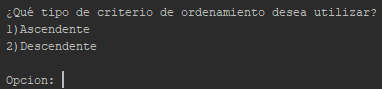
\includegraphics[height=2cm]{Imágenes/Poli2.png}
\caption{\textit{Submenú de selección para el criterio de ordenamiento.}}
\label{fig:Poli2}
\end{figure}

En caso de que se introduzca una opción entera no presente en el submenú, el programá imprimirá un error en pantalla y regresará al menú inicial.

\begin{figure}[h!]
\centering
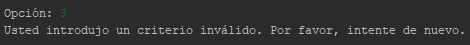
\includegraphics[height=1.25cm]{Imágenes/Poli3.png}
\caption{\textit{Submenú de selección para el criterio de ordenamiento.}}
\label{fig:Poli3}
\end{figure}

Es importante destacar que este método de ordenamiento \textbf{únicamente} ordena los números de cuenta presentes en cada clave del archivo a leer.

\subsection{Ejecución}

\noindent Una vez seleccionada la opción deseada, el ordenamiento Radix iniciará su ejecución, creando una simulación de estructuras \textit{FI-FO} y realizando un proceso de vaciado sobre un archivo llamado \textit{"nombreDelArchivo"Sorted.txt} de forma iterativa. Finalmente, el programa imprimirá en pantalla las claves ordenadas de acuerdo al criterio seleccionado.

\begin{figure}[h!]
\centering
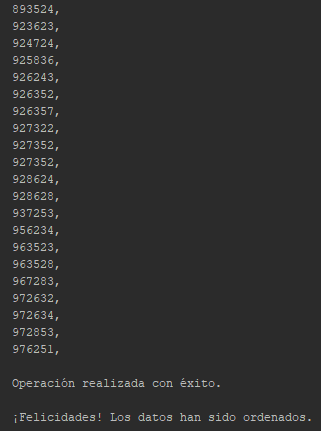
\includegraphics[height=9.25cm]{Imágenes/Radix1.png}
\caption{\textit{Salida obtenida con un archivo de 100 claves ordenadas de forma ascendente.}}
\label{fig:Radix1}
\end{figure}

Puede verificarse el resultado en el contenido del archivo \textit{"nombreDelArchivo"Sorted.txt} generado en la carpeta \textit{Archivos}; el cuál contiene las claves ordenadas por Número de cuenta. 

\begin{figure}[h!]
\centering
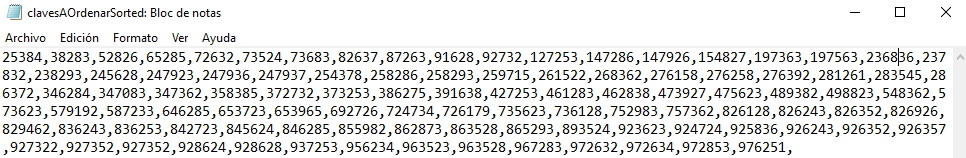
\includegraphics[height=2.7cm]{Imágenes/Radix2.png}
\caption{\textit{Contenido ordenado del archivo generado por la simulación de Radix}}
\label{fig:Radix2}
\end{figure}

Si se desea ordenar otro archivo con el formato correcto, únicamente deben de seguirse los pasos anteriores. Es importante señalar que, en caso de que el ordenamiento por Radix se inicie de nuevo, el programa ejecutará un recolector de basura interno que reinicializará todos los archivos auxiliares \textit{N0, N1, N2,... etc.} de la subcarpeta \textit{RadixExterno} provenientes de ejecuciones anteriores. El archivo de salida generado se mantiene sin cambios. 


\section{Mezcla Natural}

\subsection{Procedimiento previo a la ejecución}

\noindent El procedimiento a seguir corresponde de forma idéntica al descrito en la sección [\ref{section:2.1}] del manual. Driríjase a [\ref{section:2.1}] para mayor información.

\section{Ejecución}

\noindent Una vez que se haya realizado lo anterior, el programa comenzará a realizar el proceso inicial de lectura, generación de bloques y escritura para, finalmente, imprimir las claves ordenadas en pantalla.

\begin{figure}[h!]
\centering
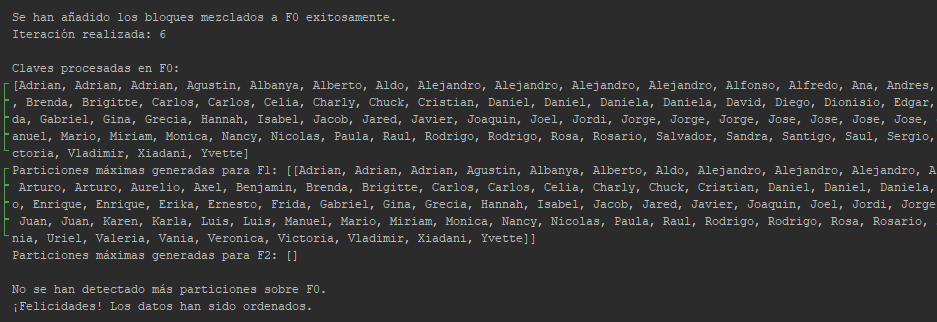
\includegraphics[height=5.8cm]{Imágenes/Mix1.png}
\caption{\textit{Salida obtenida con un archivo de 100 claves ordenadas de forma ascendente por Nombre.}}
\label{fig:Mix1}
\end{figure}

Puede verificarse el resultado en el contenido del archivo \textit{F0} generado en la carpeta \textit{Archivos $->$ MezclaNatural}; el cuál contiene las claves ordenadas en el último bloque del mismo.

\begin{figure}[h!]
\centering
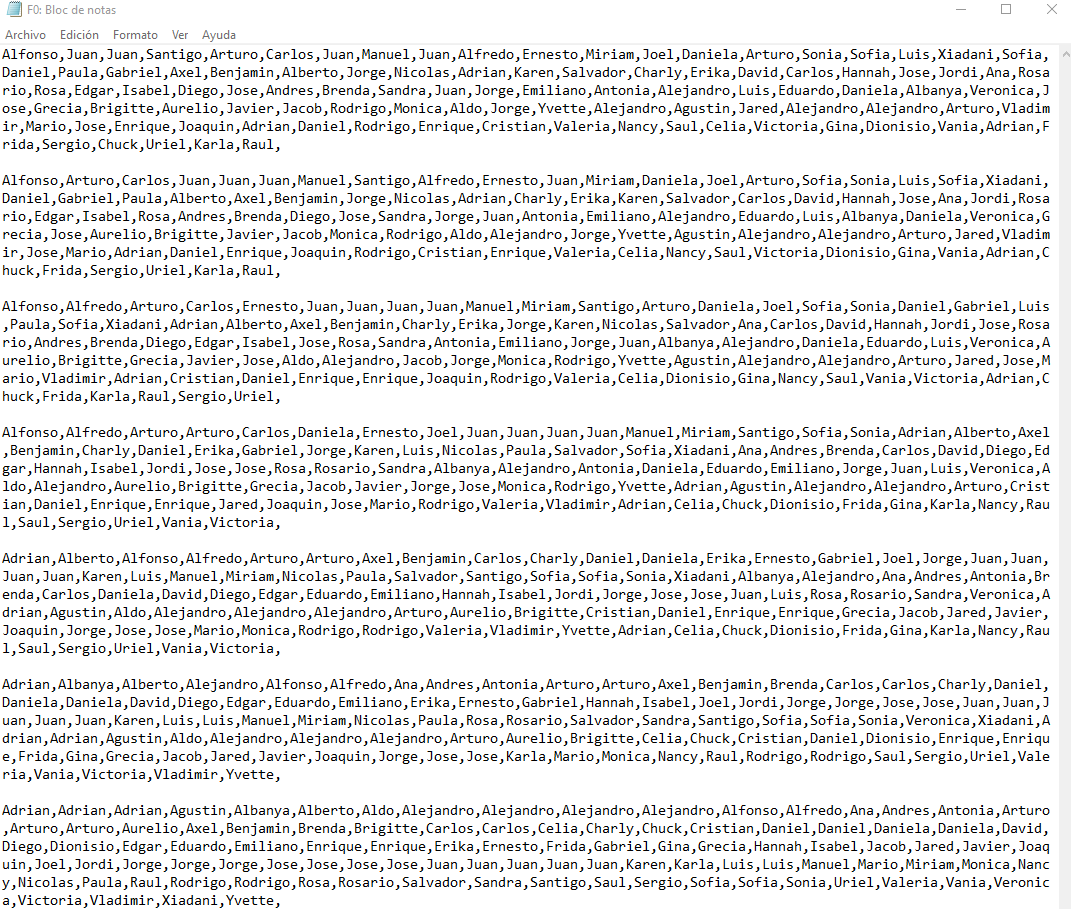
\includegraphics[height=13.8cm]{Imágenes/Mix2.png}
\caption{\textit{Contenido del archivo F0 tras ejecutar el programa.}}
\label{fig:Mix2}
\end{figure}

Si se desea ordenar otro archivo con el formato correcto, únicamente deben de seguirse los pasos anteriores. Es importante señalar que, en caso de que el ordenamiento por Mezcla Natural se inicie de nuevo, el programa ejecutará un recolector de basura interno que reinicializará los archivos \textit{F0, F1, y F2} de la subcarpeta \textit{MezclaNatural} provenientes de ejecuciones anteriores.

Cabe señalar que este método de ordenamiento hace uso de dos archivos generados automáticamente en la carpeta del proyecto: es importante \textbf{no eliminarlos} para garantizar la estabilidad del programa.

\begin{figure}[h!]
\centering
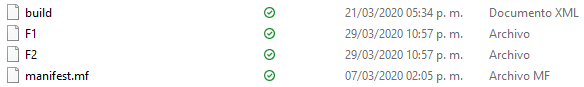
\includegraphics[height=2.3cm]{Imágenes/Mix3.png}
\caption{\textit{Archivos F1 y F2 generados en la carpeta del proyecto.}}
\label{fig:Mix2}
\end{figure}

\pagebreak

\section{Consideraciones adicionales}

\begin{itemize}
\item Se asume que el archivo introducido contiene el formato correcto para las claves. Por tanto, no se asegura una correcta ejecución en caso de presentarse errores de formato en el archivo $.txt$ seleccionado.

\item El programa únicamente ha sido probado  y ejecutado con éxito en el sistema operativo de $Windows$ $10$: no se asegura su ejecución en otras plataformas.

\item Los métodos de ordenamiento recuperan y ordenan \textbf{únicamente} el campo seleccionado de las claves, sin incluir los campos restantes durante el proceso.


\end{itemize}



\centering\vspace*{\fill} \LaTeX{}
\end{document}